\documentclass[a4paper,12pt,twoside,openany]{report}

\usepackage{titlesec}
\usepackage[T1]{fontenc}
\usepackage[utf8]{inputenc}
\usepackage[a4paper,left=3cm,right=2cm,top=2.5cm,bottom=2.5cm]{geometry}
\usepackage{hyperref}
\usepackage{array}
\newcommand{\wiki}[1]{https://pl.wikipedia.org/wiki/Teksel}

\newcommand{\DICOM}[0]{\mbox{DICOM}\xspace}

\def\zerospace{\hspace{0px}}
\def\scopedots{\zerospace::\zerospace}

\def\sokarprefix{Sokar\scopedots}
\newcommand{\sokarclass}[1]{\textit{\sokarprefix#1}}
\newcommand{\sokarfunction}[2]{\textit{\sokarprefix#1\scopedots#2()}}

\def\gdcmprefix{gdcm\scopedots}
\def\gdcmdocurl{http://gdcm.sourceforge.net/html}
\newcommand{\gdcmclass}[1]{\textit{\href{\gdcmdocurl/classgdcm_1_1#1.html}{\gdcmprefix#1}}}
\newcommand{\gdcmfunction}[2]{\textit{\href{\gdcmdocurl/classgdcm_1_1#1.html\##2}{\gdcmprefix#1\scopedots#2()}}}

\def\qtprefix{Qt\scopedots}
\def\qtdocurl{https://doc.qt.io/qt-5}
\newcommand{\qtclass}[1]{\textit{\lowercase{\href{\qtdocurl/#1.html}}{\qtprefix#1}}}
\newcommand{\qtfunction}[2]{\textit{\lowercase{\href{\qtdocurl/#1.html\##2}}{\qtprefix#1\scopedots#2()}}}

\def\stdprefix{std\scopedots}
\newcommand{\stdclass}[2]{\href{https://en.cppreference.com/w/cpp/#2}{\stdprefix#1}}

\newcommand{\dicomvr}[1]{VR:#1}

\def\dicomtagprefix{{\small$^\text{Dicom}_\text{Tag}$}\xspace}
\def\dicomtagurl#1{\url{https://duckduckgo.com/?q=!ducky+#1+site\3Adicom.innolitics.com}}
\newcommand{\dicomtag}[3]{\href{https://duckduckgo.com/?q=!ducky+DICOM+Tag+#1+(#2,#3)+site\%3Adicom.innolitics.com}{\dicomtagprefix#1 (0x#2, 0x#3)}}

\newenvironment{conditions}
{\par\vspace{\abovedisplayskip}\noindent\begin{tabular}{>{$}l<{$} @{${}={}$} l}}
        {\end{tabular}\par\vspace{\belowdisplayskip}}

\def\quotett#1{\enquote{\texttt{#1}}}
\def\cppcode#1{{\color{blue}\texttt{#1}}}
\def\keyword#1{{\textbf{#1}}}
\def\dataword#1{{\color{gray}\enquote{\texttt{#1}}}}

% \renewcommand\paragraph{%
%     \@startsection{paragraph}{4}{0mm}%
%        {-\baselineskip}%
%        {.5\baselineskip}%
%        {\normalfont\normalsize\bfseries}}


\newcommand{\fromEng}[1]{(ang. \textit{#1})}


\newenvironment{infobox}[1][]
{\begin{mdframed}[
            frametitle={#1},
            skipabove=\baselineskip plus 2pt minus 1pt,
            skipbelow=\baselineskip plus 2pt minus 1pt,
            frametitleaboveskip= 7pt,
            frametitlebelowskip= 7pt,
            linewidth=1pt,
            linecolor=black,
            frametitlerule=false,
            frametitlebackgroundcolor=blue!10,
            backgroundcolor=blue!10,
            roundcorner=7pt,
            nobreak=true
        ]}
        {\end{mdframed}}

\newenvironment{zeroindent}
{\par\setlength{\parindent}{0pt}}
{\par}


\def\qtclassExplanations{
    \begin{infobox}
        \begin{zeroindent}
            W dokumencie są wielokrotnie zawarte odniesienia do klas z biblioteki Qt.
            Dlatego, aby zwiększyć czytelność pracy, została zastosowana konwencja poprzedzania klas z biblioteki Qt przedrostkiem \textit{\qtprefix}, który jest za razem przestrzenią nazw.
            Przykład poniżej:

            \begin{center}
                \qtclass{QObject}
            \end{center}

            Wszystkie funkcje wewnątrz klas są oznaczone następująco:

            \begin{center}
                \qtfunction{QObject}{connect}
            \end{center}

            Dodatkowo w dokumencie PDF klikając na nazwę klasy użytkownik zostanie przekierowany do oficjalnej dokumentacji Qt znajdującej się pod adresem \url{\qtdocurl}.
        \end{zeroindent}
    \end{infobox}
}

\def\gdcmclassExplanations{
    \begin{infobox}
        \begin{zeroindent}
            W dokumencie są wielokrotnie zawarte odniesienia do klas z biblioteki GDCM.
            Dlatego, aby zwiększyć czytelność pracy, została zastosowana konwencja poprzedzania klas z biblioteki Qt przedrostkiem \textit{\gdcmprefix}, który za razem jest przestrzenią nazw biblioteki.
            Przykład poniżej:

            \begin{center}
                \gdcmclass{ImageReader}
            \end{center}

            Wszystkie funkcje wewnątrz klas są oznaczone następująco:

            \begin{center}
                \gdcmfunction{ImageReader}{GetImage}
            \end{center}

            Dodatkowo w dokumencie PDF można kliknąć na nazwę klasy i użytkownik zostanie przekierowany do oficjalnej dokumentacji GDCM znajdującej się pod adresem \url{\gdcmdocurl}.
        \end{zeroindent}
    \end{infobox}
}

\def\sokarclassExplanations{
    \begin{infobox}
        \begin{zeroindent}
            W dokumencie są wielokrotnie zawarte odniesienia do klas z przeglądarki obrazów.
            Dlatego, aby zwiększyć czytelność pracy, została zastosowana konwencja poprzedzania klas z aplikacji przedrostkiem \textit{\sokarprefix}, który za razem jest przestrzenią nazw programu.
            Przykład poniżej:

            \begin{center}
                \sokarclass{DataConverter}
            \end{center}

            Wszystkie funkcje wewnątrz klas są oznaczone następująco:

            \begin{center}
                \sokarfunction{DataConverter}{toString}
            \end{center}

            Dodatkowo w dokumencie PDF można kliknąć na nazwę klasy i użytkownik zostanie przekierowany do TU WYMYŚLIĆ DO CZEGO
        \end{zeroindent}
    \end{infobox}
}

\def\dicomtagExplanations{
    \begin{infobox}
        \begin{zeroindent}
            W dokumencie są wielokrotnie zawarte odniesienia do znaczników \DICOM.
            Dlatego aby zwiększyć czytelność pracy, została zastosowana konwencja poprzedzania znaczników przedrostkiem \dicomtagprefix i sufiksem składającym się z numeru grupy i elementu grupy zapisanych heksadecymalnie.
            Przykład poniżej:

            \begin{center}
                \dicomtag{PatientID}{0010}{0020}
            \end{center}

            Oznacza to, że jest to znacznik o słowie kluczowym \enquote{PatientID}, numerze grupy $10_{16}$ i numerze elementu $20_{16}$. 

            Wyrażenie \enquote{informacja ta zawarta w znaczniku \dots} będzie oznaczało, że ta informacja znajduje się w elemencie danych o znaczniku.

            Dodatkowo w dokumencie PDF można kliknąć na nazwę klasy i użytkownik zostanie przekierowany do strony \url{https://dicom.innolitics.com/ciods} poprzez wyszukiwarkę DuckDuckGo, na której znajduje się przeglądarka znaczników \DICOM.
        \end{zeroindent}
    \end{infobox}
}

\def\dicomRetired{
    \begin{infobox}
        \begin{zeroindent}
            Wiele elementów danych lub wartości zostały wycofane ze standardu \DICOM w wersji 3.0.
            Oznaczane są jako wycofane \fromEng{retired}.
            Można dalej wspierać ich obsługę w celach wstecznej kompatybilności, ale nie jest to wymagane.
        \end{zeroindent}
    \end{infobox}
}

% Aby komendy nie wychodziły poza margines
% \sloppy 

\inputencoding{utf8}

\def\utfMaleSign{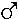
\includegraphics[height=1em]{utf8char/malesign.pdf}}
\def\utfFemaleSign{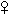
\includegraphics[height=1em]{utf8char/femalesign.pdf}}

\title{Wieloplatformowa przeglądarka obrazów DICOM w C++}

\author{Adam Jędrzejowski}
\nrindeksu{277417}

\opiekun{prof. nzw. dr hab. inż. Waldemar Smolik}
\terminwykonania{30 lutego 2019}
\rok{2019}

\miasto{Warszawa}
\uczelnia{POLITECHNIKA WARSZAWSKA}
\wydzial{Wydział Elektroniki i Technik Informacyjnych Politechniki Warszawskiej}
\instytut{Instytut Radioelektroniki i Technik Multimedialnych}
\zaklad{Zakład Elektroniki Jądrowej i Medycznej}
\kierunekstudiow{Elektronika}

\def\keywords{DICOM; przeglądarka DICOM; obrazy; obrazowanie; C++; Qt; GDCM; programowanie}
\def\keywordsEng{DICOM; DICOM viewer; images; imaging; C++; Qt; GDCM; programing}

% Ustawienie metadanych pdfu
\makeatletter
\hypersetup{
    unicode=true,
    pdfauthor={\@author},
    pdftitle={\@title},
    pdfsubject={Praca Inżynierska},
    pdfkeywords={\keywords},
    pdfproducer={\@author},
    pdfcreator={\@author}
}
\makeatother

\opinie{%
    \input{opiniaopiekuna.tex}
    \newpage
    \input{recenzja.tex}
}

\streszczenia{
    \newpage
    \begin{center}
\large \bf
\thetitle
\end{center}

Praca składa się z sześciu rozdziałów: wstęp; obrazowanie diagnostyczne w medycynie; biblioteki i narzędzia; implementacja; kompilacja; podsumowanie.
Wstęp jest powierzchownym wprowadzeniem do tematu i celu pracy.
\par
W drugim rozdziale jest opisane zagadnienie problemowe związane z obrazami w medycznie.
Wymieniono techniki diagnostyczne oraz ich podstawowe różnice między sobą.
Przedstawiono parametry jakie cyfrowy obraz medycyny posiada.
Opisano prezentacje obrazów medycznych.
Wyjaśniono czym są przeglądarki obrazów, jakie funkcje mogą posiadać i jakie kryteria wyróżniono do ich porównywania.
Opisano format zapisu cyfrowych obrazów medycznych, standard \DICOM.
\par
Trzeci rozdział opisuje biblioteki i narzędzie użyte w czasie pisania pracy inżynierskiej.
Wyjaśniono cele użycia narzędzia CMake i jego zalety.
Opisano bibliotekę Qt, jej możliwości, drzewa obiektów implementowane przez nią i sposób konstrukcji programowania zdarzeniowego w niej zawartego.
Przedstawiono i uzasadniono wybór biblioteki GDCM jako biblioteki do obsługi i wczytywania plików \DICOM.
\par
W czwartym rozdziale przedstawiono sposób implementacji pracy.
Określono przewidywany zakres implementowanych funkcji oprogramowania.
Opisano graficzny interfejs użytkownika i jego funkcje oraz ogólną funkcjonalność programu.
Wyjaśniono powierzchownie projekt struktury obiektowej programu.
Następnie szczegółowo opisano strukturę danych wraz z klasami C++.
Tam gdzie była możliwość załączono diagramu UML.
Opisano wszystkie algorytmy przetwarzania danych w celu lepszej wizualizacji obrazu.
\par
W piątym rozdziale opisano przebieg kompilacji kodu źródłowego.
\par
Prace zakończono podsumowaniem i wnioskami.

\bigskip
{\noindent\bf Słowa kluczowe:} \keywords

\vfill
    \newpage
    \begin{center}
\large \bf
Multi-platform DICOM image viewer in C++
\end{center}


The work consists of six chapters: introduction, diagnostic imaging, libraries and tools, implementation, compilation and summary.
The first chapter is an introduction to the subject and the purpose of the work.
\par
The second chapter describes problems that are related to images in medicine.
Diagnostic techniques and their basic differences are listed in this part.
There are presented the parameters of digital imagines in medicine.
In addition the presentations of the images are described and it is explained what image viewers are.
Their functions are depicted.
The format for recording digital medical images, DICOM standard, is described.
\par
The third chapter describes the libraries and tools that were used to write the engineering work.
The purpose of using the CMake tool and its advantages are explained.
The Qt library, its capabilities, object trees implemented by it and the way of programming construction have been described for the events contained in it.
The choice of the GDCM library was presented and justified as a library for handling  and loading DICOM files.
\par
The fourth chapter presents the way in which the work is implemented.
The expected range of the implemented functions of the software has been determined.
The graphical user interface and its program functions are described.
The design of the object structure of the program has been explained.
The structure of the data, together with the C++ classes is then described in details.
Where it was possibile a UML diagram was included.
All data processing algorithms are described for better  visualization of the images.
\par
The fifth chapter describes the process of compilation of the source code.

\bigskip
{\noindent\bf Keywords:} \keywordsEng

\vfill


}

\begin{document}

\maketitle

\chapter{Wstęp}
W dzisiejszych czasach obrazowanie diagnostyczne odgrywa kluczową rolę w medycynie.
Obrazy medyczne pomagają lekarzom w podejmowaniu decyzji w sprawie dalszych losów pacjenta.
Nie można pozwolić aby błąd techniczny wpłynął negatywnie na zdrowie lub życie pacjenta.
Dlatego tak bardzo ważnym aspektem obrazowania jest jego dokładność, rzetelność, niezawodność oraz powtarzalność.

Diagnostyka obrazowa lub obrazowanie medyczne to dział diagnostyki medycznej zajmujący się tworzeniem i zbieraniem obrazów ludzkiego ciała za pomocą różnych rodzaju oddziaływań fizycznych.
Obrazowe techniki diagnostyczne to techniki i procesy tworzenia wizualnych reprezentacji wnętrza obiektu do analizy medycznej.
A także wizualne przedstawienie funkcjonowania narządów lub tkanek (fizjologia) w czasie, np. bicie serca.
Głównym celem obrazowanie medycznego jest ujawnienie wewnętrznych struktur ciała.
Obrazowanie medyczne pozwala również na agregacje danych o normalnej anatomii i fizjologii i ich zapisywania, w celu poźniejszej identyfikacji patologii poprzez porównanie jej ze zdrowymi narządami.

Proces obrazowania diagnostycznego można podzielić na dwa główne etapy, pierwszy to wykonanie pomiarów na pacjencie, a drugi to analiza badania przez personel medyczny i decyzja o podjęciu działań.

Wygląd pierwszego etapu, który jest wykonywany najczęściej przez technika, jest zależny od techniki badania.
Technika badania to sposób na wejście w oddziaływanie fizyczne z ciałem pacjenta a następnie, a następnie na agregacji, czyli zbierania, danych pomiarowych.
Przykładami najbardziej popularnych badań są: radiografia, tomografia rentgenowska, obrazowanie metodą rezonansu magnetycznego, ultrasonografia, scyntygrafia, tomografia SPECT oraz tomografii PET.
Każda z wymienionych technik jest szerzej opisana w sekcji \ref{sec:basic-imaging-technics}.
Podczas badania zapisywanie są też wszystkie parametry dotyczące badania oraz tego w jakich warunkach zostało przeprowadzone.
Parametrami badania, są na przykład dane pozwalające zidentyfikować pacjenta w sposób jednoznaczny oraz jego płeć, date urodzenia, wiek w trakcie badania, sposób ułożenia ciała w urządzeniu pomiarowym.
Parametrem badania jest też model urządzenia, unikalny identyfikator urządzenia, nazwę producenta, date badania, date ostatniego przeglądu urządzenia oraz dane personalne osoby wykonującej badanie.

Na końcu tego procesu, wszystkie dane oraz parametry są zapisywane do pliku o formacie zgodnym ze standardem DICOM.
DICOM definiuje między innymi format zapisu danych i parametrów obrazowania w pliku w postaci cyfrowej.
Standard DICOM został opracowany przez dwie organizacje American College of Radiology (w skrócie ACR) i National Electrical Manufacturers Association (w skrócie NEMA) i opublikowany w swojej ostatecznej wersji w 1993.
W obecnym czasie jest to jedyny wiodący standard zapisu w obrazowaniu medycznym.

Drugi etap, czyli analiza danych i parametrów badania przez personel medyczny, sprowadza się do wyświetlenia danych i parametrów badania w taki sposób aby były zrozumiane i miały wartość diagnostyczną.
Nie jest to trywialny proces i posiada wiele aspektów.
Standard DICOM przewiduje praktyczną możliwość zapisania danych i parametrów w jakiejkolwiek formie z jakiejkolwiek techniki obrazowania.
Sprawia to, że po wczytaniu parametrów badania i ich analizie należy podjąć decyzje w jaki sposób mamy je wyświetlić użytkownikowi.
Wszystkie aspekty analizy dokonywanej przez program będą wyjaśnione w dalszych częściach dokumentu.

%rozpendówka o przetwarzaniu

Dlatego celem tej pracy inżynierskiej jest zrobienie niezawodnej przeglądarki działającej niezależnie od platformy i mogącej obsłużyć wiele typów obrazów medycznych.
Implementacje takiego rozwiązania, można zrealizować na wiele sposobów.

Możliwość uruchomienia na wielu platformach można uzyskać w wiele różnych sposobów.
Pierwszym rozwiązaniem z jest napisanie oprogramowania w środowisku, który pozwala na uruchomienie na wielu platformach.
Do takich należą Java firmy Oracle, która po skompilowaniu, tworzy jednolity kod bajtowy, który może być uruchomiany na każdej platformie na której działa maszyna wirtualna Javy.
Jednakże takie rozwiązanie sprawia, że nie jesteśmy wstanie osiągnąć pełnego potencjału obliczeniowego maszyny przez pewien poziom wirtualizacji.

Drugim rozwiązaniem jest napisanie jednolitego kodu, który można skompilować do kodu natywnego na każdą z docelowych platform.
Taką możliwość daje C++, którego kod wynikowy, posiada wysoką wydajnością z bezpośrednim dostępem do zasobów sprzętowych i funkcji systemowych, łatwością dodawania innych bibliotek, napisanych w innych niż języku niż C++.

Wybrany został drugi sposób ponieważ został w pewnym sensie narzucony przez tytuł pracy ale daje też większą możliwość wykorzystania możliwości obliczeniowych dzisiejszych komputerów.

Do pisania programu zostały wykorzystane dwie biblioteki. Qt do tworzenia interfejsu graficznego w stylu obecnej platformy. Oraz Grassroots DICOM library(w skrócie GDCM) do obsługi plików DICOM.



\chapter{Obrazowanie diagnostyczne w medycynie}

\section{Obrazowe techniki diagnostyczne}
Istnieje wiele technik obrazowania wykorzystujące różne zjawiska fizyczne zachodzące w materii.
Podstawowe techniki obrazowania medycznego to:
\label{sec:basic-imaging-technics}
\begin{itemize}
    \item Radiografia - RTG

    Radiografia to najstarsza i najbardziej rozpoznawalna technika obrazowania.
    Pierwsze zdjęcie analogowe zostało wykonane przez Röntgena w 1896 roku.
    Polega na transmisji promieniowania X przez badany obiekt, a następnie detekcji tego promieniowania za obiektem badanym.
    Promieniowanie za obiektem jest funkcją współczynnika osłabiania promieniowania rentgenowskiego dla materii znajdującej się na drodze tego promieniowania.
    Wyróżniamy dwa typy radiografii: analogową i cyfrową.
    Radiografia analogowa wykorzystująca naświetlanie filmów światłoczułych odchodzi powoli w zapomnienie ze względu na koszt i uciążliwość wywoływania filmów.
    \todo {WS: powtórzenie z analogówki; jakie dwa typy detektorów są stosowane? }
		W radiografii cyfrowej obrazowana jest ilość promieniowania X przenikające przez badany obiekt.
    
		\todo {WS podać ogólne cechy obrazu!!!; }
		Kontrast zależy od położenia obiektu między źródłem a detektorem (położenie optymalne), napięcie anodowe, filtracja, grubość okładek wzmacniających.
    \todo {WS: masło jest maślane; }
		Rozdzielczość zależy od rozdzielczości detektora i rozmiaru ogniska lampy.
    
    W standardzie DICOM radiografia cyfrowa jest oznaczana jako \quotett{RT}.

    \item Tomografia komputerowa (Computer Tomography - CT)
    
    \todo {agregacja?! }Akwizycja w tomografii komputerowej jest podobna do badania RTG, ale w CT wykonujemy wiele pomiarów w różnych pozycjach względem obiektu badanego i pod różnym kątem.
		W tomografii komputerowej podobnie jak w radiografii wykorzystuje się promieniowanie X do pomiaru projekcji (stąd inna nazwa tomografia rentgenowska). W wybranej płaszczyźnie dokonuje się pomiarów projekcji po liniach biegnących pod różnym kątem i w różnych odległościach od badanego obiektu. Przekrój obiektu jest rekonstruowany numerycznie na podstawie zmierzonych projekcji projekcji.
    \todo {tworzymy tworzący? }
		Następnie z tych pomiarów tworzymy obraz przez zastosowanie odpowiednich algorytmów tworzących obraz.
    Rejestrujemy współczynnik osłabienia promieniowania rentgenowskiego przez badany obiekt.
\todo {WS: to już było i jest bez większego znaczenia dla pracy; jakie są obrazy? rozdzielczość przestrzenna, próbkowanie, kwantyzacja? }
    Kontrast zależy od rozmiarów szczegółów badanego obiektu, napięcie anodowe, przyłożone masy (prąd katodowy i czas akwizycji).\todo {jakie mAs-y? prąd na lampie? }
    Rozdzielczość zależy od geometrii pomiaru, rozmiaru ogniska lampy rentgenowskiej, przestrzenna rozdzielczość matrycy detektora, liczby detektorów, dyskretyzację i filtru rekonstrukcyjnego.

    W standardzie DICOM technika jest oznaczana skrótowcem \quotett{CT}.

    \item Obrazowanie metodą rezonansu magnetycznego - MRI

    Sposób tworzenie obrazu MRI jest wysoce skomplikowanym procesem i ciężko opisać go w kilku zdaniach.
		\todo {to zależy od sekwencji! są obrazy PD, T1 i T2; }Obrazowana jest sumaryczna gęstość atomów wodoru (protonów) w badanym obiekcie.
    Kontrast zależy od gęstości protonów, czasu relaksacji podłużnej i poprzecznej, prędkości przepływu płynu.
    \todo {są obrazy statyczne ale też dynamiczne ; są też obrazy pokazujące funkcje (fMRI); te są pokazywane w innej skali barwnej}
		Rozdzielczość zależy od parametrów skanera (rozmiar woksela).
    
    W standardzie DICOM modalność rezonansu magnetycznego jest oznaczana jako \quotett{MR}.
    
    \item Ultrasonografia
    
    Jest to badanie, które wszyscy kojarzą z badaniem płodu podczas ciąży z obrazem w kształcie łuku na, którym nic nie widać.\todo {usunąć to zdanie} 
    Badanie ultrasonograficzne polega na wygenerowaniu fali akustycznej o wysokich częstotliwości, a następnie wprowadzeniu jej do ciała pacjenta.\todo {niefortunne 'wprowadzenie'; tu powinno by c coś o odbiciu} 
    Następnie nasłuchuje się echa po tej fali.
    Obrazowana jest odbita fala ultradźwiękowa, osłabienia po odbiciach, zmienna częstotliwość i opóźnienie w czasie.\todo {od czago zależy położenie, a od czego wielkość sygnału}
    Kontrast zależy od częstotliwości fali, głębokości badanego obiektu, ilości piezoelektryków w głowicy, obrazowanej struktury.
    Rozdzielczość zależy od czasu trwania impulsu zaburzenia oraz od szerokości wiązki ultradźwiękowej (powierzchnia czynna przetworników).

    W standardzie DICOM obraz ultrasonograficzny jest oznaczana jako \quotett{US}.\todo {mamy też obrazy doplerowskie; jak są zapisywane w DICOM?}

    \item Scyntygrafia
    
    Obrazowa technika diagnostyczna z gałęzi medycyny nuklearnej.
    Polega na wprowadzenia do organizmu \todo {to nie są ciała obce, środków chemicznych} radiofarmaceutyków znakowanych izotopem, \todo {izotop, którym znakowany jest farmacuetyk ma tę cechę}charakteryzującym się krótkim czasem rozpadu i powinowactwem chemicznym z badanymi organami.
    Następnie wykrywanie rozpadów zachodzących w ciele poprzez rejestracje promieniowania wytwarzanego podczas rozpadu, a następnie przedstawienie to w formie graficznej. \todo {detekcja}
    Kontrast zależy od czasu trwania pomiaru, oraz od aktywności wstrzykniętego radiofarmaceutyka.
    Rozdzielczość zależy od ułożenia \todo {ułożenia???} i możliwości rozdzielczej \todo {znowu masło maślane} kamer scyntylacyjnych, zwanymi także scyntykamerami, gammakamerami lub kamerami Angera.

    W standardzie DICOM obraz scyntygraficzny jest oznaczana jako \quotett{NM}.

    Radiofarmaceutyki to związki chemiczne zawierające radioizotop.

    \item Tomografia SPECT
    
    Technika obrazowania  z gałęzi medycyny nuklearnej, w której rejestruje się promieniowanie powstające rozpadu gamma.
    Źródłem promieniowania(fotonów) jest podany pacjentowi radiofarmaceutyk, ulegająca rozpadowi gamma.
    Rejestrujemy fotony powstające podczas anihilacji pozytonów.
    Kontrast zależy od wydajności detektorów, odległość detektora od obiektu oraz położenie obiektu.
    Na rozdzielczość ma wpływ przestrzenna rozdzielczość matrycy detektora, liczby detektorów.

    W standardzie DICOM obraz ultrasonograficzny jest oznaczana jako \quotett{PT}.

    \item Tomografii PET
    
    Technika obrazowania  z gałęzi medycyny nuklearnej. w której rejestruje się promieniowanie powstające podczas anihilacji pozytonów (antyelektronów).
    Źródłem promieniowania(pozytonów) jest podana pacjentowi substancja promieniotwórcza, ulegająca rozpadowi beta plus.
    Rejestrujemy fotony powstające podczas anihilacji pozytonów.
    Kontrast zależy od wydajności detektorów, odległość detektora od obiektu oraz położenie obiektu.
    Na rozdzielczość ma wpływ przestrzenna rozdzielczość matrycy detektora, liczby detektorów.

    W standardzie DICOM obraz ultrasonograficzny jest oznaczana jako \quotett{PT}.
    
\end{itemize}

Istnieją też techniki, które są połączeniem kilku innych technik.
Takie jak:
\begin{itemize}
    \item PET-CT, PET/CT - połączenie PET z wielorzędowym tomografem komputerowym
    \item PET-MRI, PET/MRI - połączenie PET z rezonansem magnetycznym
\end{itemize}

Standard DICOM nazywa techniki obrazowania modalnościami(z ang. modality).

\section{Parametry obrazów}
\subsection{Podstawowe parametry obrazu cyfrowego}

\dicomtagExplanations

\par
Każdy obraz cyfrowy jest matrycą pikseli o ustalonych rozmiarach.
W przypadku standardu \DICOM obrazy są matrycami wokseli, posiadającymi wysokość (zapisaną w \dicomtag{Rows}{0028}{0010}) oraz szerokość (zapisaną w \dicomtag{Columns}{0028}{0011}).
Do poprawnej interpretacji znaczenia macierzy służy znacznik \dicomtag{Photometric Interpretation}{0028}{0004}, informujący o fotometrycznym znaczeniu wokseli.
Standard \DICOM definiuje następujące wartości tego tagu (wraz z wyjaśnieniem):
\begin{itemize}
    \item \dataword{MONOCHROME1} i \dataword{MONOCHROME2} --- ta wartość woksela odwzorowuje skale monochromatyczną, odpowiednio od jasnego do ciemnego i od ciemnego do jasnego.

    \item \dataword{PALETTE COLOR} --- ta wartość woksela jest używana jako indeks w każdej z tabel wyszukiwania kolorów palety czerwonej, niebieskiej i zielonej.
          Palety mają swoje własne tagi.
          Wartość raczej rzadka i nie spotykana.

    \item \dataword{RGB} --- oznacza, że woksel jest trzy-kanałowym pikselem RGB (kanały: czerwony, zielony i niebieski).

    \item \dataword{HSV} \fromEng{Hue Saturation Value} --- woksel reprezentuje piksel w modelu przestrzeni barw zaproponowany w 1978 roku przez Alveya Raya Smitha.
          Model ten nawiązuje do sposobu w jakim widzi oko człowieka.
          Wartość wycofana.

    \item \dataword{ARGB} --- ta wartość woksela to piksel RGB z dodatkowym kanałem przezroczystości.
          Wartość wycofana.

    \item \dataword{CMYK} --- ten woksel to piksel w modelu czterech podstawowych kolorów farb drukarskich stosowanych powszechnie w druku wielobarwnym w poligrafii: cyjan, magenta, żółty, czarny.
          Wartość wycofana.

    \item \dataword{YBR\_FULL} --- ten woksel to piksel w modelu przestrzeni barw nazwanej YC\textsubscript{b}C\textsubscript{r}.

          Dodatkowo standard zdefiniował pochodne tej wartości: \dataword{YBR\_FULL\_422}, \dataword{YBR\_PARTIAL\_422}, \dataword{YBR\_PARTIAL\_420}, \dataword{YBR\_ICT}, \dataword{YBR\_RCT}, ale wszystkie są już wycofane.
\end{itemize}

\dicomRetired

\par
Kwantyzacja obrazu, czyli informacja mówiąca o tym ile poziomów na obrazie jest zapisanych w czterech znacznikach:
\begin{itemize}
    \item \dicomtag{Bits Allocated}{0028}{0100} --- informuje na jak wiele bitów zostało zaalokowancyh do zapisania jednego piksela
    \item \dicomtag{Bits Stored}{0028}{0101} --- informuje jak wiele bitów z zaalokowanych posiada wartość piksela
    \item \dicomtag{High Bit}{0028}{0102} --- informuje gdzie znajduje się najstarszy bit
    \item \dicomtag{Pixel Representation}{0028}{0103} --- informuje czy poziomy są ze znakiem czy bez
\end{itemize}

\par
Obraz \DICOM również zawiera w sobie informacje o próbkowaniu.
Z uwagi na to, że próbkowanie wygląda inaczej w każdej technice, standard posiada oddzielne tagi informujące o próbkowaniu dla każdej techniki.
Próbkowanie poszczególnych technik opisałem w sekcji \ref{sec:basic-imaging-technics}.

% \subsection{Wartość diagnostyczna obrazu}

% W obrazowaniu medycznym chodzi o wyciągnięcie wniosków z obrazów i postawienie diagnozy.
% Jest to kluczowy element obrazowania.
% Ocena wartości diagnostycznej to złożone zagadnienie z teorii hipotez statystycznych.
% Brak możliwości stwierdzenia co na obrazie się znajduje, stawia sens takiego obrazowania pod znakiem zapytania.
% Poco nam obraz w 4K na, którym można zobaczyć wyraźne plamy niczego.

% Wartość diagnostyczną można określić na podstawie następujących parametrów
% \begin{itemize}
%     \item Jakości obrazu

%           Parametry jakościowe obrazów są szczegółowo opisane w sekcji \ref{sec:image-quality}

%     \item Warunków obserwacji obrazu

%           W brew pozorom warunki obserwacji mają kluczowe znaczenie dla wartości diagnostycznej.
%           Jeżeli będziemy mieli dobry obraz, który wyświetlimy na budżetowym monitorze RGB, który w rzeczywistości posiada 6-bitowe kanały RGB i tworzy odcienie za pomocą techniki dithering'u, to niewiele zobaczymy.

%     \item wiarygodności diagnostycznej obrazów

%     \item charakterystyki pracy lekarza-specjalisty

% \end{itemize}

\subsection{Kontrast}

Jedną z wielu definicji kontrastu jest kontrast Michelsona wyrażony wzorem:
\[\frac{I_{max}-I_{min}}{I_{max}+I_{min}}\]
gdzie $I_{max}$ i $I_{min}$ to najwyższa i najniższa wartość luminancji.

\subsection{Rozdzielczość}

\subsubsection*{Przestrzenna}

\par
Rozdzielczość przestrzenna obrazu to najmniejsza odległość między dwoma punktami obrazu, które można rozróżnić.
Jest ona silnie związana z kontrastem obrazu za pomocą funkcji przenoszenia modulacji (MTF –-- Modulation Transfer Function).
Jest to krzywa ukazująca degradację kontrastowości w miarę zwiększania częstotliwości przestrzennej okresowego wzorca.
Funkcję MTF można wyznaczyć używając rozbieżnych tarcz rozdzielczości przestrzennej lub, w pewnych warunkach, przy pomocy norm wielopręcikowych.
W radiografii rozdzielczość określa się zazwyczaj jako liczbę równoległych linii, czarnych i białych, które można rozróżnić ma 1 milimetrze obrazu(paralinie na milimetr).

\par
Rozdzielczość przestrzenna jest zależna od kontrastu obrazu.
Zależność ta jest inna dla każdej techniki.

\subsubsection*{Czasowa}

Każdy pomiar wymaga pewnego czasu pobierania danych.
W nie których przypadkach ważna jest również zmiany zachodzące w organizmie w czasie wykonywania badania.
Rozdzielczość czasowa, jest istotna w obrazach dynamicznych, np. angioMR.
Kiedy mamy pomiar dokonywany w określonym czasie i ustalone są markery czasowe.
Rozdzielczość czasowa jest definiowana jako odległość w czasie od dwóch klatek obrazowania.

\subsection{Stosunek sygnału do szumu (SNR)}

Rodzaj i poziom szumu zależy od techniki obrazowania.
Stosunek sygnału ma decydujący wpływ na widoczności obiektów, kontrast oraz percepcję szczegółów w obrazie.

\subsection{Poziom artefaktów}

Artefakty to zjawiska fałszujące obraz poprzez tworzenie nie istniejących struktur w obrazie.
Jest to problem występujący w różnych technikach obrazowania.
Najbardziej znanymi artefaktami są np. w badaniu USG tak zwany warkocz komety w przypadku obiektów o wysokiej różnicy impedancji w stosunku do otoczenia.

\subsection{Poziom zniekształceń przestrzennych}

Zniekształcenia przestrzenne powstają w wyniku geometrycznego ułożenia i kształtu obiektu badanego oraz aparatu pomiarowego.
Przykładem takiego zniekształcenia mogą być różne powiększenia obiektów zależne od głębokości ich ułożenia w USG, zmiana pozycji pacjenta(przez ruchy klatki piersiowej w czasie badania), czy deformacja obrazu spowodowana zmianami rozkładu pola magnetycznego przez metalowe obiekty w znajdujące się w tym samym pomieszczeniu w przypadku badań MRI.



\section{Prezentacja obrazów medycznych}

\par
W celu przeglądania i porównywania należy posiadać jakieś narzędzie do wyświetlenia w sposób poprawny, najlepiej jednym i tym samym programem.
\par
Standard DICOM przewiduje sposób prezentacji danych administracyjnych i danych związanych z rejestracją badania, ajk wyświetlać obrazy radiologiczne i obrazy TK, obrazy scyntylacyjne, itd.

\subsection{Przeglądarki obrazów}

Przeglądarki obrazów to programy należące do kategorii przeglądarki plików.
Zwykłe przeglądarki obrazów takich jak jpg, png lub gif wyświetlają obraz w takiej postaci jakiej jest zapisany, oczywiście najpierw przeprowadzają dekompresje obrazu.
W przypadku obrazów medycznych najczęściej nie mamy do czynienia z danymi reprezentującymi kolory w spektrum światła widzialnego.
Przeglądarka obrazów DICOM musi wygenerować kolorowy obraz z danych na podstawie parametrów obrazu.

\subsection{Funkcje przeglądarek obrazów}

Wyróżniono 26 kryteriów do porównywania przeglądarek w postaci „tak” lub „nie”, podzielonych na 5 grup, platformy, interfejsu, wsparcie, obrazowanie dwu i trój wymiarowego.
Kryteria te w jasny sposób pozwalają na ocenę praktycznych aspektów użytkowania przeglądarki.

\subsubsection{Platforma}

Samodzielność, aplikacje samodzielne są zaprojektowane tak, aby nie wymagały żadnego dodatkowego sprzętu fizycznego bądź infrastruktury do poprawnego działania(np. systemu Windows oraz serwisów przez niego dostarczanych).
Rozwiązania sieciowe, określają czy aplikacja jest usługą sieciową i można z przeglądarki korzystać jak ze strony WWW.
Wieloplatformowość, możliwość uruchomienia ich na różnych systemach operacyjnych Linux/MacOS/Windows
Rozwiązania mobilne, możliwość używania na urządzeniach mobilnych takich jak telefon.

\subsubsection{Interfejs}

Przeglądarka powinna mieć możliwość komunikacji z interfejsami innych systemów.
Podstawowe interfejsy sieciowe to: C-STORE SCP DICOM C-STORE, C-STORE SCU, Query-Retrieve, WADO, Parameter Transfer.

\subsubsection{Wsparcie techniczne}

Dokumentacja, dostępność pisemnej dokumentacji oprogramowania (np. podręczniki lub strony internetowej).
Wsparcie przez pocztę internetową, możliwość porozumienia się z twórcą lub opiekunem oprogramowania.
Forum, możliwość pytania się społeczności o opinie i ich wymiana.
Wiki, strona internetowa w formacie Wikipedii dostępna dla użytkownika.

\subsubsection{Obrazowanie dwu-wymiarowe}

Przewijanie(\fromEng{scroll}), proces wyświetlania obrazów, można poprawić dzięki zmniejszeniu interakcji z klawiaturą oraz myszką. Można to osiągnąć na przykład, oferując możliwość przejścia do następnego lub poprzedniego obrazu przez przesunięcie kółkiem myszy lub używając przycisków góra/dół na klawiaturze.
Metadane, przeglądania powinna obejmować analizowanie i wyświetlanie metadanych obiektów DICOM, powinna obejmować wyświetlanie rozdzielczości obrazu, badanie (np. identyfikator podmiotu) oraz znaczniki DICOM specyficzne dla dostawcy (np. specjalne ustawienie urządzenia rejestrującego).
Warstwa informacyjna, najważniejsze informacje powinny powinny być wizualizowane w oknie wyświetlacza jako nakładka na obraz.
Na przykład aktualna pozycja lub nazwa podmiotu wykonującego badanie.
Okienkowanie (okna cyfrowe), sposób zamiany danych na skale szarości, okienkowanie jest opisane w sekcji \ref{sec:windowing}.
Pseudo-kolorowanie obrazu, tabele (LUT, \fromEng{LookUpTable}) odwzorowujące szare wartości obrazu na pseudo-kolory, poprawiaja one czytelność obrazu.
Histogram, histogramy wizualizują wystąpienia i rozkład wartości kolorów na obrazach, pozwalają opisywać istotne cechy obrazu
Wymiarowanie, możliwości rysowania bądź zaznaczania linii lub innych kształtów do analizy i wyznaczania odległości w jednostkach długości na obrazie.
Jest to możliwe gdyż nagłówki pliku DICOM zawierają parametry sprzętowe urządzenia (np. ilość pikseli na centymetr).
Adnotacje(opisy), które były wytworzone przez personel medyczny powinny być zapisywane w odpowiedni sposób w pliku.

\subsubsection{Obrazowanie trój-wymiarowe}

Rekonstrukcja wtórna, zwykle dane dotyczące objętości medycznej są gromadzone wzdłuż jednej osi ciała (np. poprzecznej).
W wielu przypadkach ważne jest przeglądanie danych w innych kierunkach (np. strzałkowych lub czołowych), aby poprawić wizualizację niektórych struktur.
W tym celu należy zapewnić funkcjonalność rekonstrukcji osi pomocniczej na podstawie kierunku pierwotnego.
Plastry objętości kostki(\fromEng{Slice Cube Volume}), przekroje mogą być lepiej wyświetlane w określonej pozycji.
Funkcjonalność kostki plasterka umożliwia niezależną regulację położenia różnych osi wycinków (np. poprzecznych, strzałkowych lub czołowych) w modelu objętościowym.
Podczas tego przekroje są pokazane w osobnym oknie.
Renderowanie objętościowe – dane obrazu 3D są bezpośrednio wizualizowane jako objętość.
Użytkownik może wchodzić w interakcje z woluminem poprzez obracanie lub skalowanie.
Transfer Function(nie znam polskiej nazwy), służy do odwzorowania wartości szarości obrazów wokseli na wartości krycia typów tkanek (np. kości). Struktury obrazu pasujące do wzorców szarych wartości są podświetlone. Niewykorzystane szare wartości są wyświetlane jako
przezroczyste. Specyficzne struktury stają się lepiej widoczne.
Generowanie powierzchni, dzięki różnym algorytmom można generować powierzchnie w postaci wokselów. Reprezentacje powierzchni można również zastosować do poprawy wizualizacji niektórych struktur obrazu.

\subsection{Funkcje przeglądarki obrazów}

\subsubsection{Obsługa wielu formatów danych}

Standard DICOM przewidział możliwość zapisania danych w różnych formatach.

\subsubsection{Podstawowe operacje na obrazie}

\begin{itemize}
    \item Skalowaniu lub powiększenie.
          Możliwość powiększenia lub zmniejszenia wyświetlanego obrazu o pewny współczynnik skalujący.

    \item Przesuwanie(\fromEng{pan})
          Możliwość przesuwania obrazu o dowolny wektor.
          Przydatne gdy powiększymy obraz do takiego stopnia, że nie będzie mieścił się na ekranie lub w okienku programu.

    \item Lupa, skalowanie miejscowe
          Możliwość miejscowego powiększenia obrazu.
          Przykład użycia takiego narzędzia znajduje się na rysunku \ref{fig:wyswietlanie001}.

          \begin{figure}[!htbp]
              \centering
              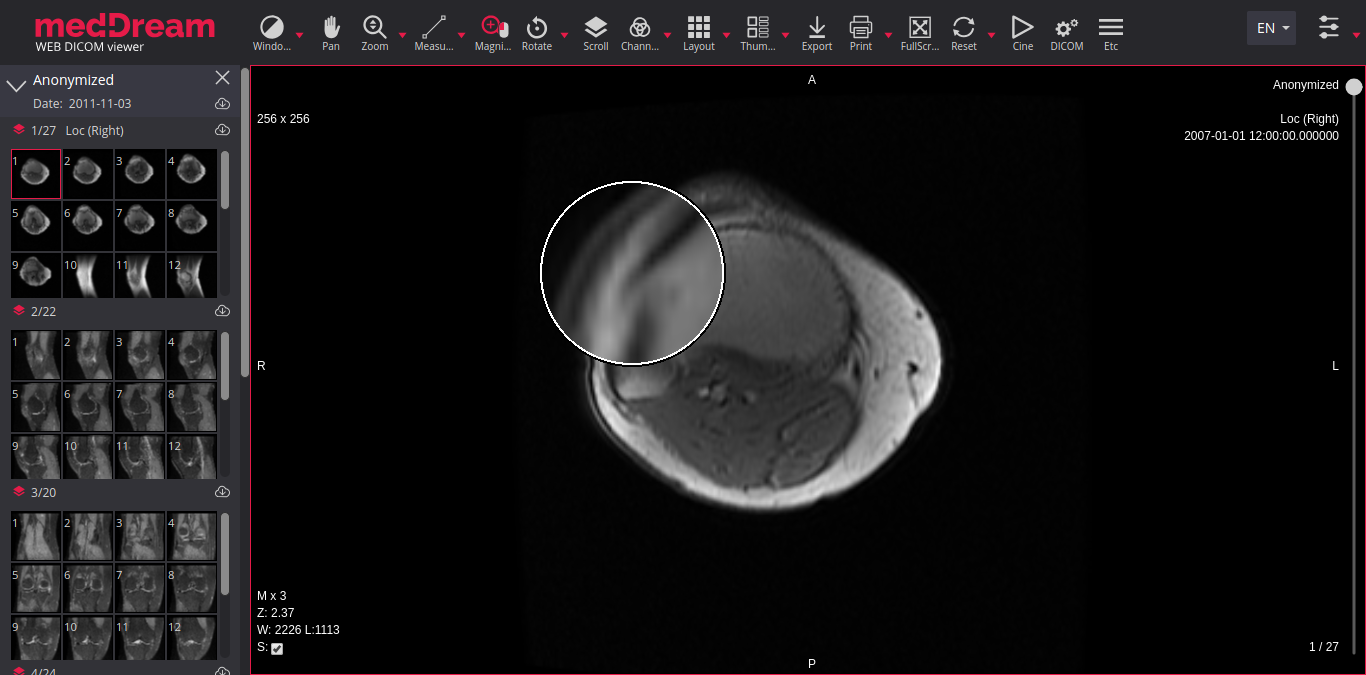
\includegraphics[width=\textwidth]{img/wyswietlanie001.png}
              \caption{Przykład narzędzia Lupa w przeglądarce \href{https://www.softneta.com/products/meddream-dicom-viewer/}{MedDream DICOM Viewer}. Zdjęcie użyte za zgodą \href{https://www.softneta.com/}{Softneta UAB}.}
              \label{fig:wyswietlanie001}
          \end{figure}

    \item Rotacja i odbicia lustrzane
          Możliwość obrócenia obrazu o zadany kąt.
          Oraz możliwość odbicia lustrzanego obrazu w dwóch osiach X i Y.

\end{itemize}

\subsubsection{Analiza parametrów w celu lepszej informacji}

\begin{itemize}
    \item Okienkowanie.
          Termin odnosi się do używania funkcji okna cyfrowego w celu zamiany obrazu danych na obraz monochromatyczny możliwy do wyświetlenia.
          Okienkowanie jest szczegółowo opisane w sekcji \ref{sec:windowing}.

    \item Maski lub nakładki(\fromEng{overlay}).
          Możliwość nałożenia maski, elementu, który będzie przysłaniał fragment obrazu w celu lepszej wizualizacji bądź ukrycie mało wartościowych obiektów, np. tła.
\end{itemize}

\subsubsection{Obsługa wielu plików}

\begin{itemize}

    \item Obsługa DICOMDIR.
          Możliwość wczytania pliku DICOMDIR i wyświetlenie struktury serii badań.

    \item Wczytanie wielu plików i ich połączenie w formie filmu.
          Możliwość wczytania wielu plików z tej samej serii, ułożenia ich według pozycji geometrycznej i wyświetlenia ich jako film.
          Czyli periodyczna podmiana obrazu na obraz następny w serii.

    \item Wyświetlanie wielu obrazów jednocześnie.
          Możliwość wyświetlenia obrazów w postaci kratki, w której każda komórka była by innym obrazem.

          Przykład wyświetlenia wielu obrazów na raz w jednym oknie znajduje się na rysunku \ref{fig:dicomviewer001}

          \begin{figure}[!htbp]
              \centering
              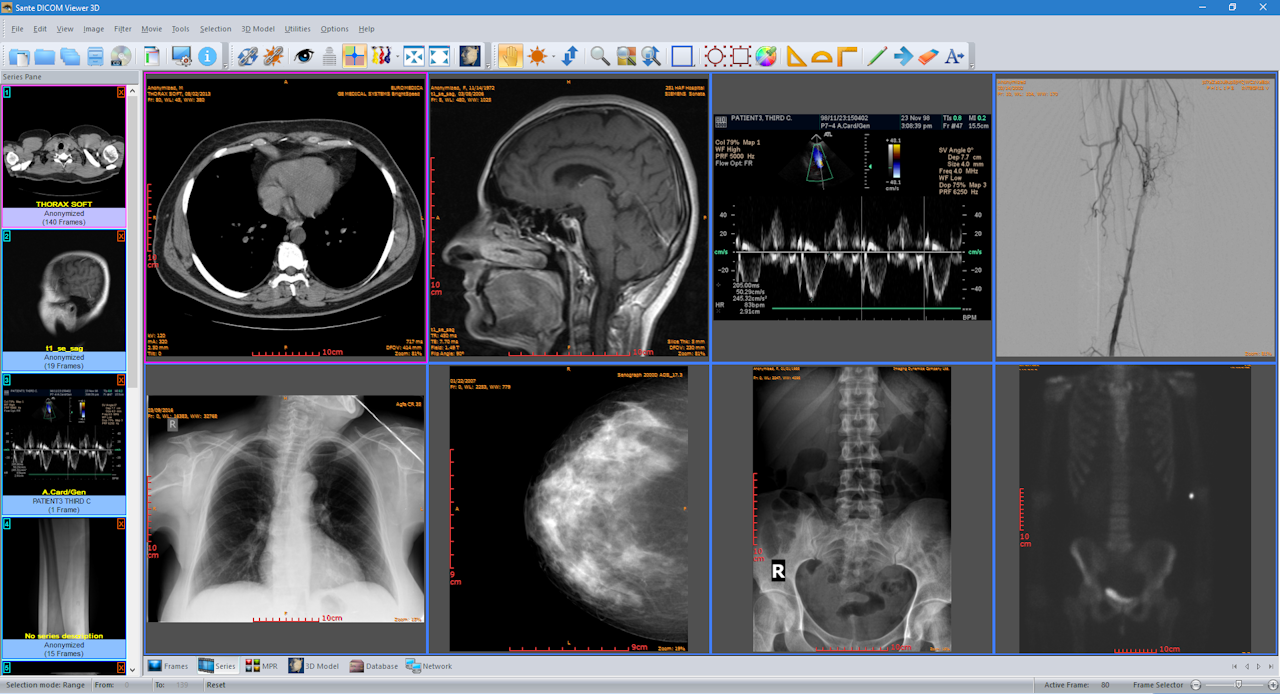
\includegraphics[width=\textwidth]{img/dicom-viewer-001.png}
              \caption{Przykład wyświetlenia wielu obrazów na raz w jednym oknie w przeglądarce \href{https://www.santesoft.com/win/sante-dicom-viewer-3d-pro/sante-dicom-viewer-3d-pro.html}{Sante DICOM Viewer 3D Pro}. Zdjęcie użyte za zgodą \href{https://www.santesoft.com/}{Santesoft}.}
              \label{fig:dicomviewer001}
          \end{figure}
\end{itemize}

\subsubsection{Generowanie obrazów woliumetrcznych}

Jeżeli mamy do dyspozycji wiele obrazów tomograficznych o znanych parametrach to możemy wczytać je, posegregować a następnie wygenerować trój-wymiarowy obiekt a następnie wyświetlić go na ekranie komputera za pomocą trójwymiarowej grafiki komputerowej.

Przykład takiego obrazu znajduje się na rysunku \ref{fig:dicomviewer002}.

\begin{figure}[!htbp]
    \centering
    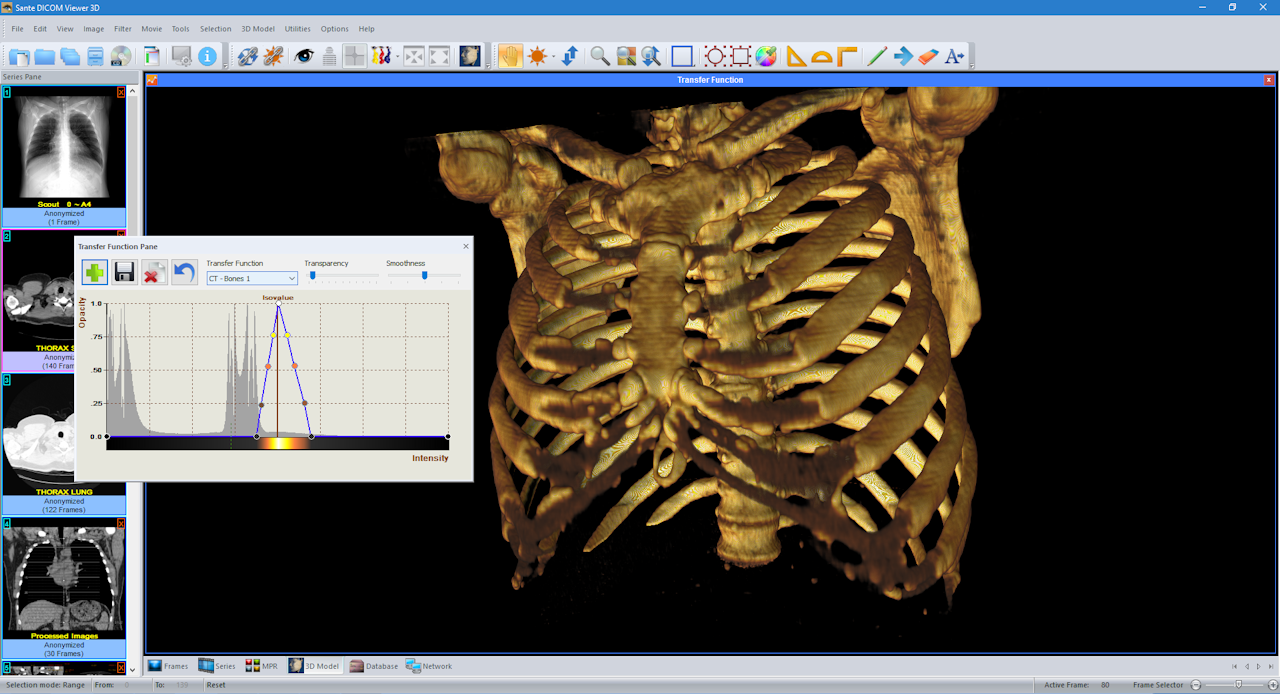
\includegraphics[width=\textwidth]{img/dicom-viewer-002.png}
    \caption{Przykład generowania obrazów 3D z wielu obrazów tomograficznych w przeglądarce \href{https://www.santesoft.com/win/sante-dicom-viewer-3d-pro/sante-dicom-viewer-3d-pro.html}{Sante DICOM Viewer 3D Pro}}
    \label{fig:dicomviewer002}
\end{figure}

\subsubsection{Analiza i przetwarznie danych}

\begin{itemize}
    \item Histogram
          Możliwość wygenerowania histogramu obrazu.

          Histogram to wykres przedstawiający dystrybucje wartości numerycznych obrazu.

    \item Mierzenie obrazu, wykonywanie pomiarów
          Możliwość zmierzenia odległości pomiędzy dwoma punktami przez lekarza lub zmierzenia wielkości/pola zadanego kształtu.

    \item Rekonstrukcja wielopłaszczyznowa.
          Obrazy tomograficzne obrazują przekroje, jeżeli parametry wielkości woksela są dostępne to istnieje możliwość wygenerowania nowego obrazu który byłby obrazem ułożonym w poprzek.

          Przykład generowania rekonstrukcja wielopłaszczyznowej jest pokazany na rysunku \ref{fig:dicomviewer003}

          \begin{figure}[!htbp]
              \centering
              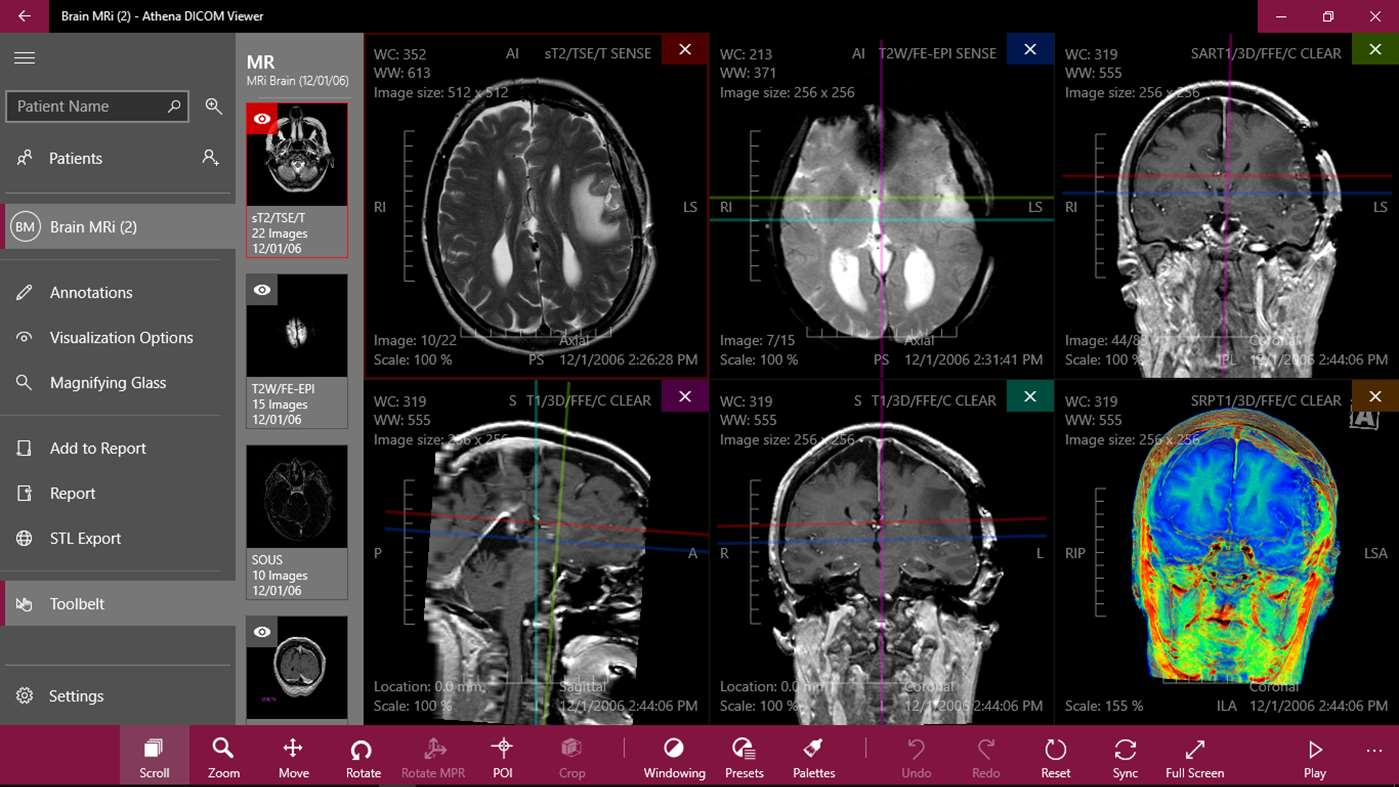
\includegraphics[width=\textwidth]{img/dicom-viewer-003.jpeg}
              \caption{Przykład rekonstrukcji wielopłaszczyznowej w przeglądarce \href{https://athenadicomviewer.com/}{Athena DICOM Viewer}. Zdjęcie użyte za zgodą \href{https://medicalharbour.com/}{Medical Harbour}.}
              \label{fig:dicomviewer003}
          \end{figure}
\end{itemize}

\subsubsection{Edycja danych}

\begin{itemize}
    \item Dodawanie nowych obiektów.
          Możliwość rysowania, dodawania figur geometrycznych lub tekstu przez lekarza i możliwość zapisu tych informacji w pliku DICOM.
          Chodzi tu głównie o szkice i notatki tworzone podczas analizy obrazu przez personel medyczny.

    \item Edycja Parametrów oraz anonimizacja danych.
          Możliwość edycji parametrów w poliku DICOM w różnych celach.
          Najczęściej funkcja jest używana do usuwania danych osobowych pacjenta w celu poźniejszej publikacji obrazu.

\end{itemize}

\section{Format cyfrowych obrazów medycznych}

\par
Pierwsze tomografy komputerowe przeżyły swój rozkwit w latach siedemdziesiątych ubiegłego wieku.
Obrazy medyczne nie były bezpośrednim wynikiem badania, a jedynie wynikiem obróbki danych pomiarowych przez komputer.
Zwyczajne pliki graficzne (jak np. jpg, png, gif), nie nadawały się do zapisu takich obrazów, ponieważ zapisywały obraz w spektrum światła widzialnego w postaci składowych RGB.
Każdy producent stosował  własny format plików, który nie był upubliczniany.

\subsection{Standard DICOM v3.0}
\input{text/obrazowanie/dicom.tex}

\subsection{Inne formaty zapisu}

\par
W tomografii komputerowej wynikiem rekonstrukcji jest macierz liczb opisujących rozkład przestrzenny współczynnika osłabiania promieniowania.
Ze względu na aspekty prawne i medyczne, niezwykle istotną rzeczą jest zapis oryginalnych danych numerycznych. Ze tego powodu producenci sprzętu wprowadzają własne formaty plików cyfrowych.
W plikach tych oprócz numerycznych danych obrazowych zapisane są parametry warunków akwizycji itp.



\chapter{Biblioteki i narzędzia}



\section*{CMake}
\par
CMake to wieloplatformowe narzędzie do automatycznego zarządzania procesem kompilacji programu.
Jest to niezależne od kompilatora narzędzie pozwalające napisać jeden plik, z którego można wygenerować odpowiednie pliki budowania dla dowolnej platformy.
\par
Z uwagi na to, że projekt musi mieć możliwość kompilacji na 3 platformy CMake jest idealnym rozwiązaniem.
Dodatkowo starałem się wybrać biblioteki, które kompilują się za pomocą CMake.

\subsection{Przebieg kompilacji za pomocą narzędzia CMake}

\subsubsection{Linux}

\subsubsection{MacOS}

\subsubsection{Microsoft Windows}

\section*{QT}
\par
Biblioteka Qt, rozwijana przez organizacje Qt Project, jest zbiorem bibliotek i narzędzi pr programistycznych dedykowanych dla języków C++, QML i Java.
\par
Qt jest głownie znane jako biblioteka do tworzenia interfejsu graficznego, jednakże posiada ona wiele innych rozwiązań ułatwiających programowanie obiektowe i zdarzeniowe.
\par
Wybrałem Qt z uwagi na to, że posiada interfejs w C++.
Oraz kompilacja oprogramowania używającego Qt może odbywać się za pomocą dwóch narzędzi: CMake oraz dedykowanego narzędzia qmake, zrobionego specjalnie na potrzeby biblioteki Qt.
Dzięki czemu cały projekt przeglądarki używa tego samego języka oraz tego samego narzędzia zarządzania kompilacją.

\subsection{Wymowa}

\par
Według autorów, Qt powinno się czytać jak angielskie słowo \enquote{cute}, po polsku \enquote{kiut}.
Jednakże społeczność programistów nie jest co fo tego zgodna.
Ankiety zrobione na dwóch popularnych serwisach internetowych o tematyce programistycznej, pokazują, że najbardziej popularną wymową jest \enquote{Q.T.}, po polsku \enquote{ku te}.
\par
Odnośniki do przytoczonych ankiet:
\begin{itemize}
    \item \url{https://ubuntuforums.org/showthread.php?t=1605716}
    \item \url{https://www.qtcentre.org/threads/11347-How-do-you-pronounce-Qt}
\end{itemize}

\subsection{Licencja}

\par
Biblioteka Qt jest dystrybuowana w dwóch wersjach: komercyjnej i otwarto źródłowej.
Wersja otwarto źródłowa nie posiada wielu modułów, ale jest dystrybuowana na licencji \href{https://www.gnu.org/licenses/gpl.html}{GNU General Public License w wersji 3}.
Co sprawia, że bibliotekę można użyć w mojej pracy.

\subsection{Norma IEC 62304:2015}

\par
The Qt Company posiada szereg certyfikatów od FDA i UE, ułatwiające wprowadzenie produktów używających bibliotek Qt na rynek Europejski jak i Amerykański.
\par
Lista posiadanych norm:
\begin{itemize}
    \item IEC 62304:2015 (2006 + A1)
    \item IEC 61508:2010-3 7.4.4 (SIL 3)
    \item ISO 9001:2015 
\end{itemize}
Więcej informacji na temat certyfikatów można przeczytać na oficjalnej stronie Qt pod adresem \url{https://www.qt.io/qt-in-medical/}.

\subsection{Klasa QObject}

\par
Biblioteka Qt implementuje klasę \qtclass{QObect}, która jest bazą dla wszystkich obiektów Qt i wszystkie klasy współpracujące z biblioteką Qt powinny po niej dziedziczyć.
\qtclass{QObject} implementuje 2 podstawowe rzeczy: system drzewa obiektów (opisany w sekcji \ref{sec:qt-pareting}), system sygnałów (opisany w sekcji \ref{sec:qt-signals}).

\subsubsection{Drzewa obiektów}
\label{sec:qt-pareting}
\input{text/biblioteki/qt-parenting.tex}

\subsubsection{Sygnały i sloty}
\label{sec:qt-signals}
\input{text/biblioteki/qt-signlas.tex}

\subsubsection{Przykładowa klasa dziedzicząca po QObject}
\input{text/biblioteki/qt-qobject.tex}

\subsection{Graficzny interfejs użytkownika}
\label{sec:qt-gui}
\input{text/biblioteki/qt-gui.tex}

\subsection{Oddzielenie od platformy}

Biblioteka standardowa

Własne wektroy

Własne wątki


\section*{GDCM}


\subsection{Uzasadnienie wyboru}

\par
Znalezienie dobrej biblioteki do obsługi jest trudne, ponieważ jest ich bardzo dużo, a ich liczba wciąż rośnie.
Powstał portal internetowy do ich indeksowania o nazwie \enquote{I DO IMAGING}, dostępny pod adresem \url{https://idoimaging.com/programs}.
\par
Biblioteka, której poszukiwano w tej pracy powinna:
\begin{itemize}
    \item współpracować z językiem C++
    \item mieć licencję pozwalającą jej używać w potrzebnym zakresie
    \item darmowa, najlepiej otwarto źródłowa
    \item aktywnie rozwijana --- znaczna większość bibliotek charakteryzowała się tym, że była porzucona i ostatnia zmiana była wprowadzona x lat temu, a proces jej rozwoju trwał od 2 do 5 miesięcy
    \item dostępna na Linuxa, MacOS i Microsoft Windows
\end{itemize}
Ostatecznie podjęto decyzję o wyborze biblioteki o nazwie Grassroots DICOM (GDCM), dostępną pod adresem \url{http://gdcm.sourceforge.net/}.

\subsection{Opis}

\par
Przetłumaczony opis biblioteki z oficjalnej strony prezentuje się następująco:
Grassroots DICOM (GDCM) to implementacja standardu \DICOM zaprojektowanego jako open source, dzięki czemu naukowcy mogą uzyskać bezpośredni dostęp do danych klinicznych.
GDCM zawiera definicję formatu pliku i protokół komunikacji sieciowej, z których oba powinny zostać rozszerzone dla zapewnienia pełnego zestawu narzędzi badaczowi lub małemu dostawcy obrazowania medycznego w celu połączenia z istniejącą bazą danych medycznych.

\par
GDCM jest biblioteką posiadającą możliwość wczytywania, edycji i zapisu plików w formacie \DICOM.
Obsługuje ona wiele kodowań obrazów jak i protokoły sieciowe.
Jest w całości napisana w C++, a do kompilacji używa CMake.
Dzięki temu w całym programie jest używany język C++ wraz z CMake, co ułatwia zarządzanie procesem kompilacji do jednego pliku.

\par
Główną zaletą biblioteki jest dobra dokumentacja wraz z przykładami jej użycia, które okazały się kluczowe przy wyborze.
Biblioteka została napisana w sposób obiektowy z usprawnieniami zawartymi w C++, takimi jak referencje i obiekty stałe, co ułatwia jej używanie.

\subsection{Licencja}

\par 
GDCM jest wydana na licencji BSD License, Apache License V2.0, która jest kompatybilna z GPLv3
Licencja ta dopuszcza użycie kodu źródłowego zarówno na potrzeby wolnego oprogramowania, jak i własnościowego oprogramowania.


\subsection{Podstawowe klasy}
\label{sec:gdcm-classes}
\input{text/biblioteki/gdcm-classes.tex}

\subsection{Przykład użycia}
\label{sec:gdcm-use}
\input{text/biblioteki/gdcm-use.tex}




\chapter{Implementacja}

\par
Najbardziej rozpoznawalne dwie przeglądarki Osirix i Horus, posiadają swoje nazwy od bogów egipskich.
Odpowiednio od Ozyrysa, boga śmierci i Horusa, boga nieba.
Dlatego postanowiłem nazwać swoja przeglądarkę w podobny sposób: Sokar.
\par
Sokar w mitologii egipskiej to bóstwo dokonujące przyjęcia i oczyszczenia zmarłego władcy oraz przenoszący go na swej barce do niebios, patron metalurgów, rzemieślników i tragarzy (nosicieli lektyk) oraz wszelkich przewoźników.

\section{Zakres implementacji}

\par
Po analizie możliwości przeglądarek plików DICOM dostępnych na rynku postanowiłem zaimplementować następujące komponenty w mojej przeglądarce:
\begin{itemize}
    \item Obsługa obrazów bez względu na ich modalność, ale z ograniczeniem do następujących interpretacji fotometrycznej:

          \begin{itemize}
              \item \dataword{MONOCHROME1}
              \item \dataword{MONOCHROME2}
              \item \dataword{RGB}
              \item \dataword{YBR}
          \end{itemize}

    \item Przesuwanie \fromEng{pan}

    \item Skalowaniu lub powiększenie poprzez decymacje i interpolacje liniowe.

    \item Rotacja i odbicia lustrzane

    \item Okienkowanie i pseudokolorowanie, zarówno w skali szarości jak i z użyciem wielo kolorowych palet.

    \item Obsługa serii obrazów jako całości
          \begin{itemize}
              \item przegląd obrazów w serii
              \item animacje
              \item wspólne okna w skali barwnej
          \end{itemize}
\end{itemize}


\section{Wieloplatformowość}
\par
Dla uzyskania wieloplatformowości kodu źródłowego zastosowano biblioteki: GDCM i Qt.
Przestrzegano standardu C++ w standardzie ISO/IEC 14882 z 2018, w skrócie C++17.
Zapewniono procedury kompilacji na wszystkie platformy poprzez użycia narzędzia CMake.


\section{Graficzny interfejs użytkownika}
\sokarclassExplanations

\par
Po uruchomieniu programu użytkownikowi ukazuje się jedno okno (rysunek \ref{sec:gui-window}), które zawiera 3 elementy: menu (obiekt klasy \qtclass{QMenuBar}), drzewa plików (obiekt klasy \sokarclass{FileTree}), obiekt zakładek z obrazami (obiekt klasy \sokarclass{DicomTabs}).
\par
Użytkownik może otworzyć plik DICOM na trzy sposoby: z menu na górze, z drzewem ze strukturą pików i poprzez przeciągnięcie.

\section{Projekt struktury obiektowej programu}

\par
W tej sekcji wyjaśniona jest ogólna struktura programu, z pominięciem dokładnych opisów poszczególnych elementów.
Ich szczegółowy opis znajduje się w następnych sekcjach.
\par
Obiekt okna, klasy \sokarclass{MainWindow} posiada 3 elementy: menu (klasy \qtclass{QMenuBar}), drzewa plików (klasy \sokarclass{FileTree}), obiekt zakładek (klasy \sokarclass{DicomTabs}).
Zakładki obiektu zakładek są implementowane prze klasę \sokarclass{DicomView}.
Obiekt zakładki posiada abstrakcyjną kolekcję scen, implementowaną przez \sokarclass{DicomSceneSet}.
Kolekcja scen odpowiada za przechowywanie obrazów i scen, obiektów klasy \sokarclass{DicomScene}.
Sceny nie posiadają bezpośredniego dostępu do pliku, a jednie wskaźniki do odpowiednich miejsc w pamięci, gdzie obrazy są przechowywane.
Ogólny diagram klas znajduje się na rysunku \ref{fig:uml-global-sturcture}.

\begin{figure}[!htbp]
    \centering
    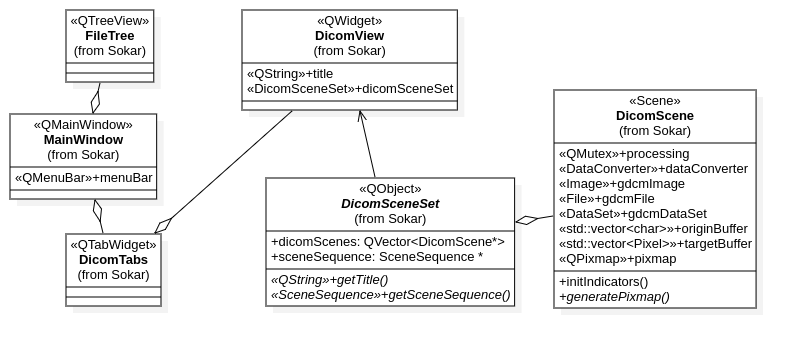
\includegraphics[width=\textwidth]{img/uml/global-sturcture.png}
    \caption{Diagram klas UML globalnej struktury programu.}
    \label{fig:uml-global-sturcture}
\end{figure}


\section{Struktury danych}

\subsection{Konwertowanie danych z znacznikach}
\input{text/implementacja/strukturydanych/conventer.tex}

\subsection{Scena}
\input{text/implementacja/strukturydanych/dicom-scene.tex}

\subsection{Kolekcje scen}
\input{text/implementacja/strukturydanych/dicom-scene-sets.tex}

\subsection{Zakładka}
\input{text/implementacja/strukturydanych/dicom-view.tex}

\subsection{Obiekt zakładek}
\input{text/implementacja/strukturydanych/dicom-tabs.tex}

\subsection{Okno główne programu}
\input{text/implementacja/strukturydanych/sokar-window.tex}


\section{Algorytmy}


\subsection{Cykl generowania obrazów}
\input{text/implementacja/algorytmy/pixmap-generate.tex}

\subsection{Generowania obrazu monochromatycznego}
\input{text/implementacja/algorytmy/pixmap-monochrome.tex}

\subsection{Tworzenie transformat i ich użycie na obrazie}
\input{text/implementacja/algorytmy/pixmap-transformat.tex}

\subsection{Ustalanie pozycji pacjenta względem sceny}
\input{text/implementacja/algorytmy/image-orientation-indicator.tex}

\section{\sokarclass{DicomView}}
\label{sec:sokar-dicomview}
Każda zakładka z obrazem lub obrazami jest implementowana przez klasę \sokarclass{DicomView}.

Interfejs graficzny \sokarclass{DicomView} wyświetla następujące elementy:
\begin{itemize}
    \item pasek narzędzi znajdujący się na górze - implementowany za pomocą klasy \sokarclass{DicomToolBar}, opisany w sekcji \ref{sec:sokar-dicomtoolbar}
    \item miejsce na scene z obrazem DICOM na środku - implementowany za pomocą klasy \sokarclass{DicomGraphics}, opisany w sekcji \ref{sec:sokar-dicomgraphics}
    \item suwak filmu w dolnej części - implementowany za pomocą klasy \sokarclass{MovieBar}, opisany w sekcji \ref{sec:sokar-moviebar}
    \item podgląd miniaturek obrazów w prawej części - implementowany za pomocą klasy \sokarclass{FrameChooser}, opisany w sekcji \ref{sec:sokar-framechooser}
\end{itemize}

Dodatkowo posiada obiekt \sokarclass{DicomSceneSet}, który jest zbiorem obrazów opisany w sekcji \ref{sec:sokar-scenesets}.
\sokarclass{DicomView} łączy zdarzenia wysyłane przez wszystkie obiekty.

Poniżej jest opisane zachowanie tych elementów:

\subsection{Elementy interfejsu graficznego}

\begin{figure}[!htbp]
    \centering
    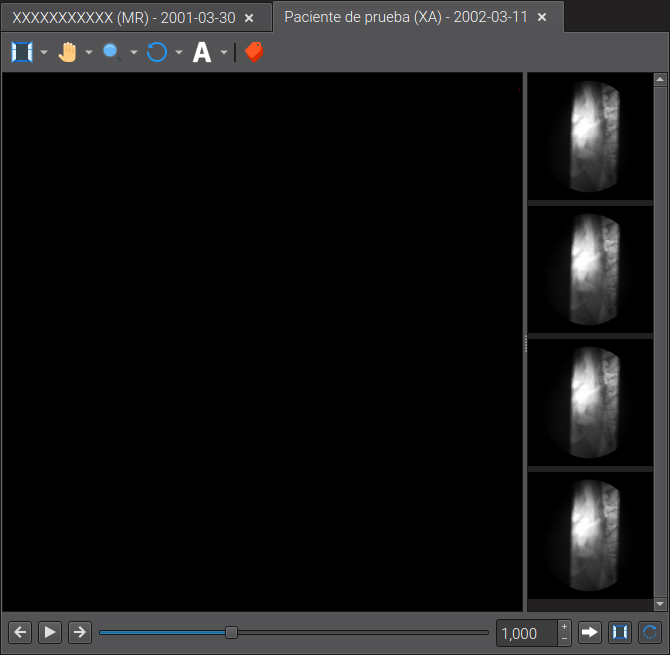
\includegraphics[width=\textwidth]{img/sokar-dicomview-001.png}
    \caption{Wygląd DicomView wraz z numeracją elementów interfejsu. Zdjęcie własne.}
    \label{fig:sokar-dicomview001}
\end{figure}

\subsubsection{\sokarclass{DicomToolBar}}
\label{sec:sokar-dicomtoolbar}
\input{text/implementacja/dicom-toolbar.tex}

\subsubsection{\sokarclass{DicomGraphics}}
\label{sec:sokar-dicomgraphics}

\subsubsection{\sokarclass{MovieBar}}
\label{sec:sokar-moviebar}

\par
Jest paskiem filmu w dolnej części \sokarclass{DicomView}.
Element graficzny ma dostęp do sekwencji scen i ukrywa swoją obecność przed użytkownikiem, kiedy w sekwencji jest tylko jedna scena.

\par
Pasek jest podzielony na trzy części: trzy przyciski znajdujące się po lewej, pasek pokazujący postępu sekwencji na środku i prządka z trzema przyciskami po prawej.

\par
Trzy lewe przyciski odpowiadają za poruszanie się po sekwencji.
Wciśniecie pierwszego przycisku (z indeksem 8 na rysunku \ref{fig:sokar-dicomview001}) powoduje zatrzymanie upływu sekwencji i wysłanie sygnału \sokarfunction{SceneSequence}{stepBackward} do sekwencji.
Wciśniecie drugiego przycisku (9) powoduje włączenie lub wyłączenie upływu sekwencji.
Wciśniecie trzeciego przycisku (10) powoduje zatrzymanie upływu sekwencji i wysłanie sygnału \sokarfunction{SceneSequence}{stepForward} do sekwencji.
\par
Pasek (11) pokazujący postępu sekwencji jest obiektem klasy \qtclass{QSlider}.
Odświeżanie paska jest wrażliwe na sygnał \sokarfunction{SceneSequence}{steped} of sekwencji.
\par
Elementy po prawej stronie definiuje parametry trybu filmowego.
Prządka (12), element do wprowadzania liczby zmiennoprzecinkowej klasy \qtclass{QDoubleSpinBox}.
Im większa wartość liczby tym klatki filmu są dłużej wyświetlane.
Drugi (13) przycisk pozwala zmienić sposób przemiatania.
Trzeci (14) przycisk wymusza tryb jednego okna dla wszystkich klatek filmu.
Jeżeli mamy załadowanych wile obrazów tego samego badania, to nie koniecznie muszą mieć to samo okno.
Dodatkowo ten tryb pozwala wprowadzić jednolite okienko dla wszystkich klatek po zmianie parametrów tego okienka na jednej klatce.
Czwarty (15) i ostatni przycisk służy do użycia jednej macierzy transformaty na wszystkich klatkach.

\paragraph*{Tryb filmowy}

\par
Tryb filmowy można aktywować jedynie wtedy gdy w sekwencji scen jest więcej niż jedna scena.
Włączenie trybu filmowego polega na stworzeniu obiektu klasy \sokarclass{MovieMode}.
Obiekt ten zapisuje wskaźnik go obecnie wyświetlanej sceny, to czy powinno być użyte to samo okno, oraz to czy powinna być używana ta sama transformata.
Następnie obiekt ten jest wysyłany do wszystkich scen w sekwencji.
Uruchamiany jest timer, obiekt klasy \qtclass{QTimer}, na czas równy czasu trwania sceny zapisanego w kroku przemnożonego przez liczbę z prządki.
Po upływie timera, wstawiana jest nowa scena za pomocą sygnały \sokarfunction{MovieBar}{setStep}, a timer jest ustawiany nan nowo.

\subsubsection{\sokarclass{FrameChooser}}
\label{sec:sokar-framechooser}

Ten element to wybór scen za pomocą ikon, implementowany przez klasę \sokarclass{DicomView}.
Element, podobnie jak pasek filmu ma dostęp do sekwencji scen i ukrywa swoją obecność przed użytkownikiem, kiedy w sekwencji jest tylko jedna scena.
Po wciśnięciu ikony jest zmieniana scena.

\section{\sokarclass{DicomTabs}}
\label{sec:sokar-dicomtabs}

\par
Jest to obiekt odpowiadający za wyświetlanie wielu obiektów \sokarclass{DicomView} w jednym okienku w formie zakładek.
Obsługuje również prośby o wczytanie nowych plików

\subsection{Segregacja plików DICOM}

\section{Okno główne programu}
\label{sec:sokar-window}

\par
Główne okno programu jest implementowane przez \sokarclass{MainWindow}.
Jest wywoływane od razu po uruchomieniu programu.
\par
Zawiera w sobie 4 elementy: menu, drzewo ze strukturą plików, obiekt z zakładkami \sokarclass{DicomTabs} i sugestie aby nie używać programu w celach medycznych w dolnej części okna.

\subsection{Drzewo plików i zakładki}

\par
W lewej części okna znajduje się element listy, implementowany przez \sokarclass{FileTree}, zawiera on w sobie model drzewa plików systemu, który z koleji jest implementowany przez klasę \qtclass{QFileSystemModel}.
Po wybraniu pliku, ścieżka jest przesyłana do obiektu z zakładkami.
\par
W środkowej części programu znajduje się obiekt z zakładkami, szczegółowo opisany w sekcji \ref{sec:sokar-dicomtabs}.

\subsection{Menu programu}
\label{sec:sokar-window-menu}

\par
W górnej części okna programu znajduje się menu, obiekt klasy \sokarclass{QMenuBar}.
Struktura Menu programu:
\begin{itemize}
    \item File
          \begin{itemize}
              \item Open --- otwiera okienko wyboru plików, implementowane przez \qtfunction{QFileDialog}{getOpenFileName}, następnie wczytuje plik
              \item Open Recent --- program zapisuje ostatnio wczytane pliki i może wczytać je ponownie z tego menu
              \item Export as --- zapisanie obrazu w formacie JPEG, BMP, GIF lub PNG.
                    Zapisywanie jest zaimplementowane przez funkcje \qtfunction{QImage}{save}, która umożliwia zapisanie obrazu do pliku.
              \item Exit --- wyjście z aplikacji
          \end{itemize}
    \item Help
          \begin{itemize}
              \item About Qt --- otwiera okno informacji o bibliotece Qt.
              Biblioteka Qt ma wbudowane takie okno w postaci \qtfunction{QMessageBox}{aboutQt}
              \item About GDCM --- otwiera okno z informacjami o bibliotece GDCM, implementowane przez funkcje \sokarfunction{About}{GDCM}
              \item About Sokar --- otwiera okno z informacjami o aplikacji, implementowane przez funkcje \sokarfunction{About}{Sokar}
          \end{itemize}
\end{itemize}



\listoffigures

\end{document}
